\chapter{Физический смысл и график функции Грина}
\section{Температурный импульс}
Функция $G(x,\xi,t)$ --- отклик на начальное распределение
$\delta(x-\xi)$ при однородных границах. Она удовлетворяет
$G_t=a^2G_{xx}-bG$, $G(0,\xi,t)=0$, $G_x(l,\xi,t)=0$ и
\[
 \lim_{t\downarrow0}\int_0^lG(x,\xi,t)\psi(x)dx=\psi(\xi),\qquad 0<\xi<l.
\]
Единичный температурный импульс не равен одному джоулю:
внесение теплоты $Q$ при объёмной теплоёмкости $c$ и сечении $S$
даёт $u=QG/(cS)$. Источник в момент $\tau$ порождает ядро
$G(x,\xi,t-\tau)$. Линейность позволяет суммировать такие отклики.
\section{Приближённое построение}
Используем первые $N=100$ мод при $l=a^2=1$, $b=0.5$, $\xi=0.4$,
$t_1=0.01$, $t_2=0.06$. Это безразмерные параметры численного примера,
а не заданные физические константы варианта.
График вычислен по спектральной формуле; внешняя картинка не требуется.
Для графика взята 81 точка $x$, а численные характеристики ниже проверены
на более густой сетке из 2001 точки.
\begin{figure}[htbp]
\centering
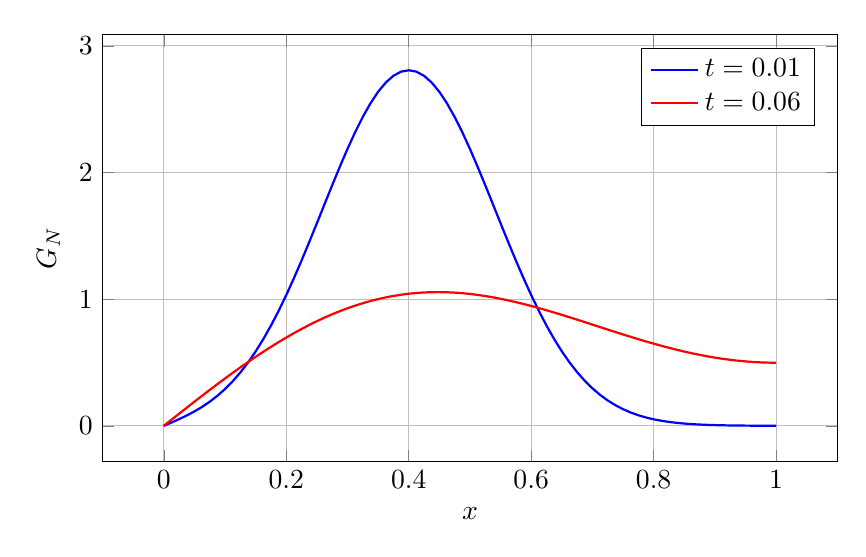
\begin{tikzpicture}
\begin{axis}[width=.9\textwidth,height=7cm,xlabel={$x$},ylabel={$G_N$},grid=major,legend pos=north east]
\addplot[blue,thick] coordinates {
(0.00000,0) (0.01250,0.0258722216228) (0.02500,0.0527481184805) (0.03750,0.0816294039483) (0.05000,0.113512707456) (0.06250,0.149384200598) (0.07500,0.190211016216) (0.08750,0.236928707166) (0.10000,0.290424254848) (0.11250,0.351514455725) (0.12500,0.420919876742) (0.13750,0.499234963358) (0.15000,0.586895288126) (0.16250,0.684143320111) (0.17500,0.790994449368) (0.18750,0.907205287304) (0.20000,1.03224645404) (0.21250,1.16528213124) (0.22500,1.3051585819) (0.23750,1.45040360341) (0.25000,1.59923848416) (0.26250,1.74960348573) (0.27500,1.8991971945) (0.28750,2.04552931422) (0.30000,2.1859856501) (0.31250,2.31790322073) (0.32500,2.4386526866) (0.33750,2.54572466095) (0.35000,2.63681602453) (0.36250,2.70991214396) (0.37500,2.76336092018) (0.38750,2.7959348808) (0.40000,2.80687806543) (0.41250,2.79593520871) (0.42500,2.7633616511) (0.43750,2.70991344265) (0.45000,2.63681817697) (0.46250,2.54572812753) (0.47500,2.43865818511) (0.48750,2.3179118509) (0.50000,2.18599907684) (0.51250,2.04555003328) (0.52500,1.89922891341) (0.53750,1.74965166412) (0.55000,1.59931109233) (0.56250,1.45051217666) (0.57500,1.30531967102) (0.58750,1.1655192775) (0.60000,1.03259285035) (0.61250,0.907707326091) (0.62500,0.791716401399) (0.63750,0.685173436949) (0.65000,0.588353671512) (0.66250,0.501283595639) (0.67500,0.423775253368) (0.68750,0.355463298809) (0.70000,0.295842809334) (0.71250,0.244306120395) (0.72500,0.200177268554) (0.73750,0.162742979426) (0.75000,0.131279489008) (0.76250,0.105074817716) (0.77500,0.0834464091688) (0.78750,0.0657542889959) (0.80000,0.0514100867091) (0.81250,0.0398823952891) (0.82500,0.0306990216056) (0.83750,0.0234467124599) (0.85000,0.0177689339833) (0.86250,0.013362245401) (0.87500,0.00997175084577) (0.88750,0.00738604340571) (0.90000,0.00543198122363) (0.91250,0.00396956214087) (0.92500,0.00288709554009) (0.93750,0.0020968106724) (0.95000,0.00153099155409) (0.96250,0.00113869008945) (0.97500,0.000883041153044) (0.98750,0.000739185041154) (1.00000,0.000692792622264)
};
\addlegendentry{$t=0.01$}
\addplot[red,thick] coordinates {
(0.00000,0) (0.01250,0.0478081373586) (0.02500,0.0955127838547) (0.03750,0.14301073166) (0.05000,0.190199339055) (0.06250,0.236976813562) (0.07500,0.283242495119) (0.08750,0.328897139215) (0.10000,0.37384319985) (0.11250,0.417985112051) (0.12500,0.461229573639) (0.13750,0.503485825763) (0.15000,0.544665931633) (0.16250,0.584685052749) (0.17500,0.623461721794) (0.18750,0.660918111224) (0.20000,0.696980296466) (0.21250,0.731578512529) (0.22500,0.764647402712) (0.23750,0.796126257997) (0.25000,0.825959245651) (0.26250,0.854095625493) (0.27500,0.880489952226) (0.28750,0.90510226225) (0.30000,0.927898243338) (0.31250,0.948849385613) (0.32500,0.967933112302) (0.33750,0.985132888836) (0.35000,1.00043830894) (0.36250,1.01384515651) (0.37500,1.0253554422) (0.38750,1.0349774138) (0.40000,1.04272553978) (0.41250,1.04862046528) (0.42500,1.05268894046) (0.43750,1.05496372103) (0.45000,1.05548344101) (0.46250,1.05429245827) (0.47500,1.05144067334) (0.48750,1.0469833223) (0.50000,1.04098074499) (0.51250,1.03349812945) (0.52500,1.02460523447) (0.53750,1.01437609155) (0.55000,1.00288868826) (0.56250,0.990224634868) (0.57500,0.976468816335) (0.58750,0.961709031782) (0.60000,0.946035623719) (0.61250,0.929541099254) (0.62500,0.912319745579) (0.63750,0.894467242022) (0.65000,0.876080270877) (0.66250,0.857256129226) (0.67500,0.838092343816) (0.68750,0.818686291025) (0.70000,0.799134823752) (0.71250,0.779533907006) (0.72500,0.759978263743) (0.73750,0.740561032403) (0.75000,0.721373437367) (0.76250,0.702504473438) (0.77500,0.684040605214) (0.78750,0.666065482087) (0.80000,0.648659669409) (0.81250,0.631900396202) (0.82500,0.615861319628) (0.83750,0.600612306302) (0.85000,0.586219230384) (0.86250,0.572743788278) (0.87500,0.560243329659) (0.88750,0.548770704483) (0.90000,0.538374125552) (0.91250,0.529097046172) (0.92500,0.520978052418) (0.93750,0.514050769516) (0.95000,0.50834378185) (0.96250,0.503880566144) (0.97500,0.500679437408) (0.98750,0.498753507282) (1.00000,0.498110654507)
};
\addlegendentry{$t=0.06$}
\end{axis}\end{tikzpicture}
\caption{Отклик на температурный импульс при двух моментах времени.}
\end{figure}
\section{Интерпретация и погрешность}
Максимумы равны приблизительно $2.806878$ и $1.055518$;
их координаты на сетке --- $0.4000$ и $0.4475$.
Диффузия расширяет возмущение, а охлаждение и потери на левом торце
уменьшают его амплитуду. Правый торец теплоизолирован.
Смещение пика обусловлено несимметричными граничными условиями.
Интегральная температура $M=\int_0^lGdx$ подчиняется балансу
\[
 M'=-a^2G_x(0,\xi,t)-bM.
\]
Метод трапеций на 2001 точке даёт $M(t_1)=0.990358$,
$M(t_2)=0.729564$. Проверка усечения отделена от ошибки сетки:
\[
 \sup_x|G-G_N|\le\frac2l e^{-bt}\sum_{n=N}^{\infty}e^{-a^2k_n^2t}.
\]
Сравнение 100 и 200 мод при этих временах не выявляет различий
в машинной точности. При $t\downarrow0$ число мод надо увеличивать.
